% Informe del Examen Interciclo · Redes Vehiculares y Heterogéneas · Universidad de Cuenca
% Plantilla IEEE Conference (IEEEtran, modo conference). Compilar: pdflatex, bibtex, pdflatex ×2.
\documentclass[conference]{IEEEtran}
\IEEEoverridecommandlockouts
\usepackage[utf8]{inputenc}
\usepackage[T1]{fontenc}
\usepackage[spanish,es-noshorthands,es-tabla,es-nodecimaldot]{babel}
\usepackage{icomma}
\usepackage{cite}
\usepackage{amsmath,amssymb}
\usepackage{graphicx}
\usepackage{booktabs}
\usepackage{array}
\usepackage{tabularx}
\usepackage{xcolor}
\usepackage{tikz}
\usetikzlibrary{arrows.meta,positioning,fit}
\usepackage{url}
\usepackage[hidelinks]{hyperref}
\newcommand{\cod}[1]{\texttt{#1}}
\def\BibTeX{{\rm B\kern-.05em{\sc i\kern-.025em b}\kern-.08em T\kern-.1667em\lower.7ex\hbox{E}\kern-.125emX}}

\begin{document}

\title{e-sert: guía al puesto libre y cobro por tiempo real de parqueo en la zona SERT del Centro Histórico de Cuenca, evaluados con SUMO y TraCI}

\author{\IEEEauthorblockN{Tyrone Novillo, Freddy López, Pablo Calle y Miguel Bermeo}
\IEEEauthorblockA{Carrera de Telecomunicaciones, Facultad de Ingeniería\\
Universidad de Cuenca, Cuenca, Ecuador\\
Redes Vehiculares y Heterogéneas · Examen Interciclo (proyecto P4)}}

\maketitle

\begin{abstract}
Buscar parqueo en el Centro Histórico de Cuenca obliga a dar vueltas, con costo en tiempo, distancia y emisiones. Este trabajo presenta e-sert, un prototipo para el Sistema de Estacionamiento Rotativo Tarifado (SERT) que guía al conductor al puesto libre, cobra por adelantado en bloques de 30 minutos, recarga saldo con la API de Payphone en modo de pruebas y cierra la sesión sola cuando un Random Forest detecta, con el GPS del teléfono, que el conductor ya va en su auto. Todo el sistema se evalúa sobre una simulación microscópica en SUMO de la red real del Centro, controlada en línea con TraCI. Como la EMOV no entregó a tiempo el inventario de puestos, se generaron 6\,194 puestos sintéticos justificados sobre 103 calles tarifadas. En 40 corridas (cinco semillas) de la hora pico, con 87,4\,\% de ocupación, la guía con la ocupación real de los puestos reduce el tiempo de búsqueda en 17,6\,\% (433 a 357\,s, $p<0{,}001$), la distancia en 16,4\,\% y el CO$_2$ de búsqueda por auto en 17,7\,\%. En cambio, una guía basada solo en lo que reportan los usuarios de la app no mejora la búsqueda, porque su mapa acierta el 57\,\% de los puestos. El clasificador elimina las falsas liberaciones que una regla de velocidad comete en 87 de cada 100 sesiones. Los resultados son simulados y se presentan como tales.
\end{abstract}

\begin{IEEEkeywords}
SUMO, TraCI, parqueo inteligente, búsqueda de parqueo, Random Forest, detección del modo de transporte, sistemas inteligentes de transporte.
\end{IEEEkeywords}

\section{Introducción}
El Centro Histórico de Cuenca concentra comercio, servicios y patrimonio en calles estrechas, la mayoría de un solo sentido. El estacionamiento en la vía se controla con el SERT, operado por la EMOV EP, que cobra 0,25~USD por media hora~\cite{concejo2012sert}. En la hora pico, cuando la ocupación supera el 85\,\%, los conductores dan vueltas a la manzana hasta encontrar un puesto. Shoup recopiló 16 estudios en los que encontrar puesto en la calle tomaba de 3,5 a 14 minutos y entre el 8 y el 74\,\% del tráfico estaba buscando parqueo~\cite{shoup2006cruising}.

La pregunta del proyecto es: \emph{si una parte de los conductores usa una app que los guía al puesto libre, ¿cuánto bajan el tiempo, la distancia y el CO$_2$ de la búsqueda, y qué hace falta para que esa mejora ocurra?} Responderla en la calle exige datos que no existen todavía, por lo que el sistema completo se evalúa sobre una simulación microscópica en SUMO~\cite{lopez2018sumo}, controlada en línea mediante TraCI~\cite{wegener2008traci}, los dos temas centrales del primer parcial de la asignatura.

Los aportes son: (i) un escenario SUMO del Centro Histórico con 610 áreas de parqueo sintéticas justificadas, intercambiables por el inventario de la EMOV sin cambiar el código; (ii) un controlador TraCI que crea los peatones de la app, emula el GPS con ruido, clasifica el movimiento y guía al puesto libre por la ruta de manejo más corta; (iii) una comparación con línea base, repeticiones e intervalos de confianza que separa el valor de la guía del valor del dato de ocupación; y (iv) un prototipo en línea con app web, pago y visor 3D.

\section{Estado del arte}
\label{sec:arte}
La Tabla~\ref{tab:arte} resume los seis artículos revisados y su diferencia con e-sert.

\textbf{Información para la búsqueda.} Di Martino \emph{et~al.}~\cite{dimartino2019comparing} compararon, con datos reales de parqueo en la calle de San Francisco, tres niveles de información para un sistema de guía: ninguna, estática (capacidad y restricciones de cada tramo) y en tiempo real (sensores fijos). Encontraron que las estrategias informadas reducen de forma significativa la búsqueda, que la información en tiempo real mejora poco sobre la estática, y que solo cuando quedan muy pocos puestos el dato en tiempo real se vuelve más valioso. Nuestro escenario está justo en ese régimen (87\,\% de ocupación) y, como se verá, el valor del dato de ocupación domina el resultado.

\textbf{Evidencia de campo.} Dalla Chiara \emph{et~al.}~\cite{dallachiara2022curb} desplegaron en Seattle una app (OpenPark) que mostraba la disponibilidad en tiempo real de la acera a repartidores, en un experimento controlado con y sin acceso a la app. Con la información, el tiempo de búsqueda bajó 27,9\,\% y la distancia 12,4\,\%. Es una medida real del orden de magnitud que buscamos; nuestro caso son autos particulares y la evaluación es simulada.

\textbf{Búsqueda y emisiones.} Xiao y Jaller~\cite{xiao2025prediction} usaron seis meses de GPS agregado de Nueva York y Los Ángeles para explicar el tiempo medio de búsqueda con un modelo de rezago espacial y propusieron un marco para predecirlo por celdas y estimar sus emisiones. Mostraron que la búsqueda se derrama espacialmente y que sus zonas críticas coinciden con puntos de alta emisión. Nosotros medimos emisiones por vehículo con el modelo HBEFA de SUMO, en lugar de inferirlas de datos agregados.

\textbf{SUMO para asignar puestos.} Alekszejenkó y Dobrowiecki~\cite{alekszejenko2022validating} propusieron un método de asignación de parqueaderos para vehículos autónomos sobre un modelo abstracto de ciudad, y lo validaron contra una simulación microscópica en SUMO de un distrito de Budapest. Comparten con este trabajo el uso de SUMO como banco de prueba de un algoritmo de asignación; difieren en que su usuario es un auto autónomo y no hay cobro ni detección de salida.

\textbf{Guía cooperativa sin infraestructura.} De Soricellis \emph{et~al.}~\cite{desoricellis2026cooperative} agregan evidencia de eventos de parqueo aportada por los vehículos participantes en mapas de calor compartidos y eligen el puesto con un puntaje que equilibra probabilidad de encontrar puesto y distancia a pie. En una campaña en SUMO, con distintas tasas de adopción, la evidencia compartida redujo la búsqueda incluso con adopción parcial, con sensibilidad a la información inicial (arranque en frío); además construyeron un prototipo con baliza BLE, app y servidor. Es el trabajo más cercano: nuestro ``mapa propio'' también se construye solo con los usuarios, pero a 87\,\% de ocupación no mejoró la búsqueda.

\textbf{Modo de transporte con el teléfono.} Castrogiovanni \emph{et~al.}~\cite{castrogiovanni2020smartphone} propusieron un marco de aprendizaje automático que, con pocos datos del teléfono, distingue transporte público de privado con buena exactitud y bajo consumo de batería, y publicaron un conjunto de datos anonimizado. Nuestro problema es más estrecho y más costoso de errar: decidir, solo con GPS, cuándo el conductor deja de caminar y vuelve a manejar, porque eso cierra el cobro.

\begin{table*}[t]
\centering
\caption{Artículos revisados (2019--2026) frente a e-sert}
\label{tab:arte}
\footnotesize
\begin{tabularx}{\textwidth}{@{}p{2.6cm}XXXX@{}}
\toprule
Trabajo & Problema & Método & Resultado & Diferencia con e-sert \\
\midrule
Di Martino \emph{et~al.} 2019~\cite{dimartino2019comparing} & Qué información sirve a un sistema de guía en la calle & Tres estrategias (sin información, estática, sensores en tiempo real) con datos reales de San Francisco & Menos búsqueda con información; el tiempo real solo ayuda cuando quedan pocos puestos & Medimos el sistema completo en SUMO; a 87\,\% de ocupación el dato real sí decide \\
Castrogiovanni \emph{et~al.} 2020~\cite{castrogiovanni2020smartphone} & Detectar transporte público o privado con el teléfono & Aprendizaje automático con pocos datos del teléfono; conjunto de datos abierto & Buena exactitud y bajo consumo de batería & Clases a pie/quieto/vehículo; la métrica es la falsa liberación del cobro \\
Alekszejenkó y Dobrowiecki 2022~\cite{alekszejenko2022validating} & Asignar parqueadero a autos autónomos & Modelo abstracto validado con SUMO en un distrito de Budapest & El modelo abstracto se valida con la simulación microscópica & Conductores humanos, cobro SERT y peatones en la simulación \\
Dalla Chiara \emph{et~al.} 2022~\cite{dallachiara2022curb} & Búsqueda de acera de repartidores & Experimento controlado con la app OpenPark en Seattle & $-27{,}9$\,\% de tiempo y $-12{,}4$\,\% de distancia de búsqueda & Autos particulares; evaluación simulada con cinco semillas \\
Xiao y Jaller 2025~\cite{xiao2025prediction} & Predecir búsqueda y emisiones & Rezago espacial y predicción por celdas con GPS agregado de NYC y LA & La búsqueda se derrama; coincide con puntos de alta emisión & CO$_2$ por vehículo con HBEFA en SUMO, con y sin app \\
De Soricellis \emph{et~al.} 2026~\cite{desoricellis2026cooperative} & Guía sin sensores en la calle & Mapas de calor con evidencia de los usuarios; SUMO con adopción parcial; prototipo BLE & Menos búsqueda incluso con adopción parcial & Con 87\,\% de ocupación, el mapa de usuarios no bastó; se cuantifica el valor del dato real \\
\bottomrule
\end{tabularx}
\end{table*}

\section{Metodología}
El proyecto sigue el lazo dato--modelo--acción--medida--visualización (Fig.~\ref{fig:arq}). Toda la simulación, el backend y la visualización corren en un servidor con Docker; el detalle de versiones está en la Sección~\ref{sec:replica}.

\begin{figure}[t]
\centering
\begin{tikzpicture}[font=\scriptsize, node distance=5mm and 14mm,
  caja/.style={draw, rounded corners=2pt, align=center, minimum height=8mm, text width=2.5cm, fill=white},
  flecha/.style={-{Stealth[length=2mm]}, thick}]
\node[caja, fill=orange!10] (sumo) {SUMO 1.12\\red del Centro, 610 áreas};
\node[caja, right=of sumo, fill=orange!10] (ctrl) {Controlador TraCI\\peatones, GPS, guía};
\node[caja, below=of sumo, fill=blue!6] (back) {Backend FastAPI\\sesiones, billetera};
\node[caja, below=of ctrl, fill=green!8] (ia) {Random Forest\\ventanas de 30\,s};
\node[caja, below=of back, fill=red!6] (app) {App web\\Payphone (pruebas)};
\node[caja, below=of ia, fill=blue!6] (visor) {Visor 3D (three.js)\\y sumo-gui (noVNC)};
\draw[flecha] ([yshift=1.5mm]ctrl.west) -- node[above]{órdenes} ([yshift=1.5mm]sumo.east);
\draw[flecha] ([yshift=-1.5mm]sumo.east) -- node[below]{estado} ([yshift=-1.5mm]ctrl.west);
\draw[flecha] (ctrl) -- (ia);
\draw[flecha] (ctrl.south west) -- (back.north east);
\draw[flecha,{Stealth[length=2mm]}-{Stealth[length=2mm]}] (back) -- (app);
\draw[flecha] (back.south east) -- (visor.north west);
\end{tikzpicture}
\caption{Arquitectura de e-sert. SUMO solo se modifica a través de TraCI; el controlador envía al backend un \emph{snapshot} por segundo y el visor lo recibe por WebSocket.}
\label{fig:arq}
\end{figure}

\subsection{Dato: red y puestos sintéticos justificados}
La red se construyó con \cod{netconvert} a partir de OpenStreetMap en el recuadro de latitudes $-2{,}905$ a $-2{,}8895$ y longitudes $-79{,}013$ a $-78{,}9945$: 985 aristas para autos, 1\,824 peatonales, 775 cruces, 129 semáforos y 90,66~km de vías. Se conservaron aceras y cruces porque el conductor de la app camina y ese recorrido es el que observa el clasificador.

La EMOV no entregó a tiempo la ubicación ni los códigos de los puestos. Siguiendo la regla del examen de datos sintéticos justificados, \cod{generar\_parkingareas.py} crea un \cod{parkingArea} por tramo de cuadra con reglas explícitas (Anexo~\ref{sec:anexo}): calles con nombre de tipo residencial, terciaria, secundaria o sin clasificar; lado derecho; 5,5~m por puesto; 8~m libres en cada esquina; tramos de al menos 12~m; y exclusión de las avenidas Huayna Cápac y Gaspar Sangurima, sin parqueo en la vía. Resultan 610 áreas con 6\,194 puestos en 103 calles (10,15 por área). Cada área recibe un código de 001 a 610. El identificador \cod{pa\_<arista>\_0} es el mismo en SUMO, el backend y la app, y todo el sistema lee \cod{puestos.csv} (id, arista, calle, capacidad, latitud, longitud): con el inventario de la EMOV solo cambia ese archivo.

\textbf{Demanda.} Autos de fondo ocupan el 80\,\% de los puestos desde el inicio; el tráfico de paso es el 40\,\% de las llegadas; los buscadores van a 12 destinos reales (mercados, plazas, iglesias) con una estadía lognormal de media 45~min y, si su puesto está lleno, siguen buscando con los \cod{rerouter} de parqueo de SUMO. La tasa de 1\,800~veh/h se calibró para una ocupación media entre 85 y 95\,\%, el rango en que buscar cuesta; la línea base dio 87,4\,\% (IC~95\,\% [87,0;~87,9]). Cada corrida simula 75~min: 15 de calentamiento y 60 de hora pico.

\subsection{Acción: el controlador TraCI}
El controlador (\cod{traci/}) avanza SUMO paso a paso (1~s) y en cada paso lee el estado y emite órdenes por TraCI (Tabla~\ref{tab:traci}). Para los experimentos se usa \cod{libsumo}, la misma interfaz enlazada en el proceso, más rápida.

\begin{table}[t]
\centering
\caption{Uso de TraCI en el controlador}
\label{tab:traci}
\scriptsize
\begin{tabularx}{\columnwidth}{@{}>{\raggedright\arraybackslash}p{4.3cm}>{\raggedright\arraybackslash}X@{}}
\toprule
Comando & Uso \\
\midrule
\cod{parkingarea.getVehicleCount} & ocupación real de cada área \\
\cod{simulation.getParking\-Starting\-VehiclesIDList} & detectar quién estacionó \\
\cod{person.add}, \cod{appendWalkingStage} & el conductor baja, camina y vuelve \\
\cod{vehicle.getPosition},\\ \cod{simulation.convertGeo} & traza para el GPS emulado \\
\cod{simulation.findRoute} & distancia de manejo a cada candidato \\
\cod{vehicle.rerouteParkingArea} & guiar al puesto elegido \\
\cod{vehicle.setParkingAreaStop} & estacionar los autos de la app \\
\cod{vehicle.isStoppedParking} & verdad de terreno de las falsas liberaciones \\
\bottomrule
\end{tabularx}
\end{table}

\textbf{GPS emulado.} La posición del auto o del peatón pasa por un ruido autocorrelacionado AR(1) con $\rho=0{,}8$ y $\sigma$ de 3 a 15~m, el rango de error del GPS urbano reportado en la literatura; cada 5~s se arma una ventana de 30~s.

\textbf{Guía.} En los experimentos, el auto con app se desvía al puesto libre más cercano a su destino. \textbf{Guía por ruta.} Para los autos de la app en línea, que no indican destino, el puesto se elige entre los 25 puestos libres más cercanos en línea recta (ocupación real menos reservas), calculando su distancia de manejo con \cod{findRoute} y probando también el carril contrario al arrancar; se toma el de menor recorrido. La versión anterior tomaba el más cercano en línea recta, que en calles de un solo sentido obligaba a dar vueltas (Sección~\ref{sec:rutas}). Si el puesto se llena mientras el auto llega, cada 5~s se reasigna con \cod{rerouteParkingArea}.

\subsection{Modelo: clasificador de movimiento}
Un Random Forest~\cite{breiman2001random} de scikit-learn~\cite{pedregosa2011scikit} (100 árboles, profundidad máxima 20, mínimo 5 muestras por hoja, pesos balanceados, \cod{random\_state}=42) clasifica cada ventana en \emph{a pie}, \emph{quieto} o \emph{vehículo} con 18 características (percentiles de velocidad, aceleración, cambio de rumbo, rectitud, desplazamiento neto, paradas). Se entrenó con 445\,607 ventanas de GeoLife~\cite{zheng2010geolife,zheng2008learning} (trazas reales; 10 usuarios reservados para prueba) y de episodios de SUMO con ruido en las posiciones. La sesión pasa a \emph{saliendo} cuando dos ventanas seguidas dicen \emph{vehículo}. La línea base es la regla del contrato: más de 8~km/h es vehículo.

\subsection{Acción en la app: reserva, cobro inmediato y pago}
La app web ofrece dos formas de registrar el puesto: \emph{buscar parqueadero cercano} (SUMO crea el auto y lo guía) o \emph{ya estacionado} (se escribe el código del puesto). En ambas el puesto queda reservado. Al llegar se eligen 30, 60, 90 o 120~min y se debita en ese instante 0,25~USD por bloque, la tarifa de la ordenanza~\cite{concejo2012sert}; a 5~min del final la app avisa y renueva sola otros 30~min hasta 120. Sin saldo, se recarga con el botón de pago de Payphone~\cite{payphone_api} en modo de pruebas: el backend prepara la transacción y la confirma con Payphone antes de acreditar.

\subsection{Medida: diseño experimental}
La búsqueda empieza cuando el auto entra a 300~m de su destino y termina al estacionar; la distancia y el CO$_2$ (modelo HBEFA de SUMO) se suman en ese lapso. La matriz cruza la penetración de la app $\{0,20,50,80\}$\,\% con dos clasificadores (regla y Random Forest) y cinco semillas: 35 corridas, más cinco de sensibilidad al 50\,\% en las que la guía usa la ocupación real de SUMO (``ocupación real''). Con números aleatorios comunes, la demanda depende solo de la semilla y el sorteo de quién tiene app es anidado, así que la única diferencia entre escenarios de una semilla es la app. Los KPI por vehículo se resumen con un IC~95\,\% \emph{bootstrap} jerárquico (semillas y vehículos, 10\,000 remuestreos); las falsas liberaciones con IC de Wilson; cada escenario se compara con la línea base con Mann-Whitney~U. El mapa ``propio'' de la app solo conoce las sesiones de sus usuarios.

\subsection{Visualización}
El visor web muestra en vivo la simulación en 3D con three.js (Fig.~\ref{fig:visor}): 5\,571 edificios de OpenStreetMap extruidos, las calles de SUMO, los puestos (verde si quedan plazas, rojo si está lleno), los autos estacionados en sus plazas y los autos en movimiento con el color de su estado; cada auto de la app lleva el nombre de su usuario. Además, \cod{sumo-gui} se controla desde el navegador mediante noVNC.

\begin{figure}[t]
\centering
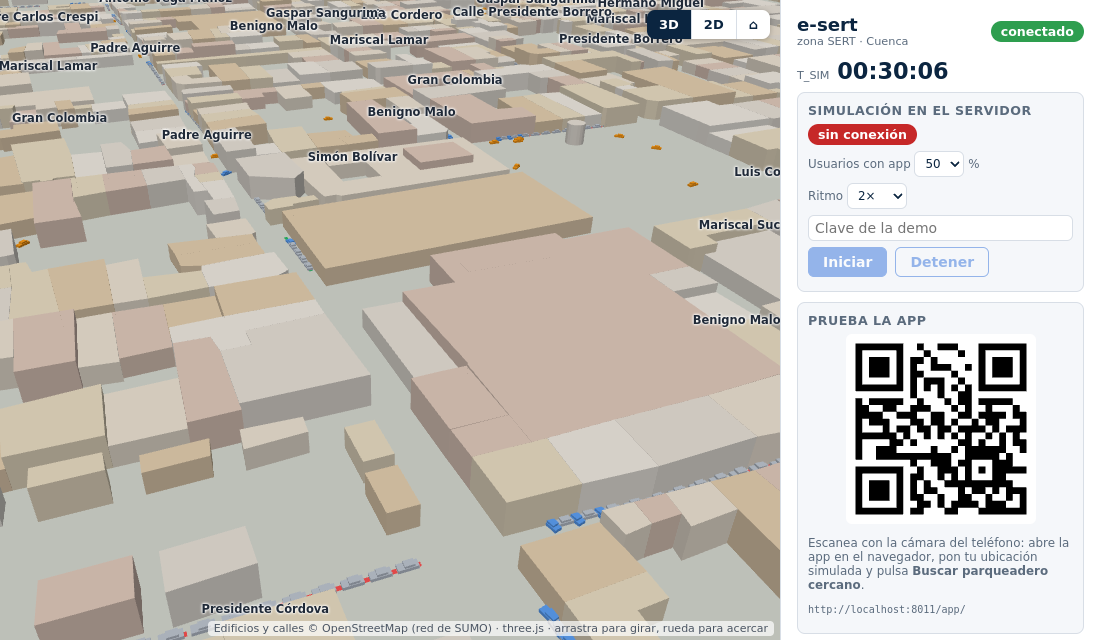
\includegraphics[width=\columnwidth]{figuras/visor3d.png}
\caption{Visor 3D en vivo: edificios, puestos punteados (verde/rojo), autos estacionados y en movimiento sobre la red de SUMO.}
\label{fig:visor}
\end{figure}

\section{Resultados}
Todas las cifras de esta sección son simuladas (SUMO, cinco semillas, unos 4\,700 buscadores por escenario). Los controles de cordura se cumplieron: los teletransportes no superaron el 0,166\,\% de los vehículos en ninguna corrida.

\subsection{Tiempo de búsqueda frente a la línea base}
La Tabla~\ref{tab:kpi} y la Fig.~\ref{fig:busqueda} muestran el resultado central. A ciegas, un auto busca 433~s y recorre 1\,456~m. Con la ocupación real, al 50\,\% de usuarios, la búsqueda baja a 357~s ($-17{,}6$\,\%, $p<0{,}001$), la distancia a 1\,217~m ($-16{,}4$\,\%) y el CO$_2$ por auto de 838 a 690~g ($-17{,}7$\,\%) (Fig.~\ref{fig:co2}). Los autos con app buscan 310~s y los que no la tienen también ganan (405~s), porque dejan de competir por los mismos puestos. En toda la zona, el CO$_2$ de búsqueda baja de 779 a 661~kg por hora pico.

Con el mapa propio, en cambio, la búsqueda no mejora: $+0{,}4$, $+1{,}3$ y $+4{,}1$\,\% al 20, 50 y 80\,\%, con intervalos que se solapan con la línea base (al 80\,\%, $p=0{,}054$). Al 50\,\%, los autos con app buscan 442~s frente a 434~s de los demás.

\begin{table}[t]
\centering
\caption{KPI de búsqueda por escenario (media e IC~95\,\%; simulado)}
\label{tab:kpi}
\scriptsize
\setlength{\tabcolsep}{2.5pt}
\begin{tabular}{@{}lrrrr@{}}
\toprule
Escenario & Búsqueda (s) [IC] & $\Delta$ & Dist.\ (m) & CO$_2$ (g) \\
\midrule
A ciegas & 433 [418; 448] & --- & 1\,456 & 838 \\
App 20\,\% & 434 [423; 446] & $+0{,}4$\,\% & 1\,445 & 845 \\
App 50\,\% & 438 [425; 451] & $+1{,}3$\,\% & 1\,468 & 853 \\
App 80\,\% & 451 [433; 470] & $+4{,}1$\,\% & 1\,450 & 880 \\
App 50\,\% ocup.\ real & \textbf{357} [344; 373] & $\mathbf{-17{,}6}$\,\% & \textbf{1\,217} & \textbf{690} \\
\bottomrule
\end{tabular}
\end{table}

\begin{figure}[t]
\centering
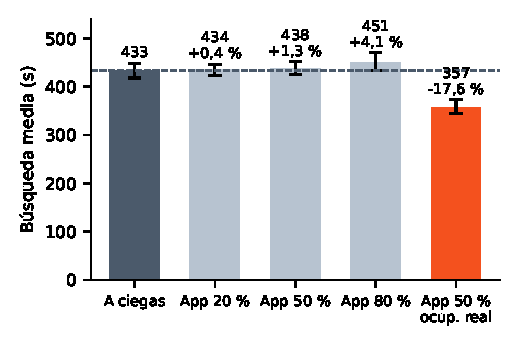
\includegraphics[width=\columnwidth]{figuras/busqueda.pdf}
\caption{Tiempo medio de búsqueda con IC~95\,\%. La línea discontinua es la búsqueda a ciegas. Datos simulados.}
\label{fig:busqueda}
\end{figure}

\begin{figure}[t]
\centering
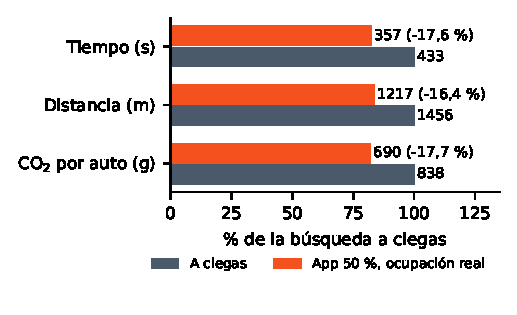
\includegraphics[width=\columnwidth]{figuras/co2.pdf}
\caption{Tiempo, distancia y CO$_2$ de búsqueda por auto, a ciegas y con la app al 50\,\% guiando con la ocupación real. Datos simulados.}
\label{fig:co2}
\end{figure}

\subsection{Cierre automático del cobro}
La Fig.~\ref{fig:falsas} compara las falsas liberaciones, es decir, sesiones cerradas mientras el auto sigue estacionado. La regla de velocidad comete 88,9, 87,2 y 86,6 por cada 100 sesiones al 20, 50 y 80\,\%, porque el error autocorrelacionado del GPS hace que un teléfono quieto parezca moverse. El Random Forest no cometió ninguna (cotas superiores de Wilson 1,31, 0,52 y 0,34). Su retardo mediano de cierre fue de 22,7, 18,8 y 18,4~s desde que el auto arranca, y el error de facturación medio pasó de $-0{,}153$ a $+0{,}018$~USD por sesión. Con usuarios de GeoLife nunca vistos, el F1 macro fue 0,872 (IC [0,818; 0,946]) frente a 0,698 de la regla; la inferencia tarda 1,35~ms (mediana).

\begin{figure}[t]
\centering
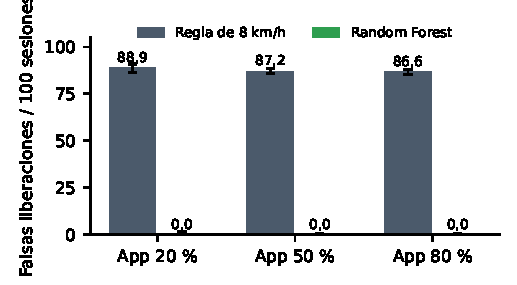
\includegraphics[width=\columnwidth]{figuras/falsas.pdf}
\caption{Falsas liberaciones por 100 sesiones (IC de Wilson~95\,\%). Datos simulados.}
\label{fig:falsas}
\end{figure}

\subsection{Elección del puesto por ruta}
\label{sec:rutas}
Para 300 puntos al azar junto a los puestos del Centro, con cerca del 85\,\% de las áreas llenas, se comparó la distancia de manejo hasta el puesto elegido por cada método (Fig.~\ref{fig:rutas}). Eligiendo el más cercano en línea recta, la media fue de 478~m (mediana 383, percentil 90 de 947~m) y 105 casos superaron los 500~m; eligiendo por ruta, la media fue de 230~m (mediana 198, percentil 90 de 410~m) y solo 18 casos superaron los 500~m.

\begin{figure}[t]
\centering
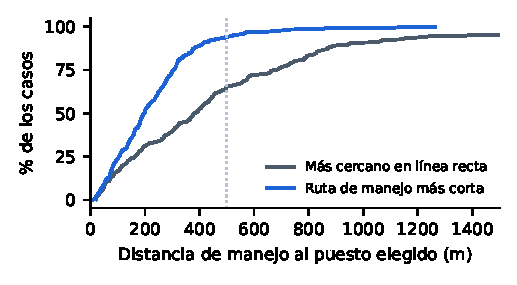
\includegraphics[width=\columnwidth]{figuras/rutas.pdf}
\caption{Distribución acumulada de la distancia de manejo al puesto elegido; 300 puntos, semilla 1. La línea punteada marca 500~m.}
\label{fig:rutas}
\end{figure}

\section{Discusión}
\textbf{El dato de ocupación decide.} La guía funciona cuando conoce la ocupación real: $-17{,}6$\,\% de búsqueda y de CO$_2$, en el orden del $-27{,}9$\,\% medido en campo por Dalla Chiara \emph{et~al.}~\cite{dallachiara2022curb}. Con un mapa construido solo por sus usuarios, la app no ve los autos sin app que ocupan casi todos los puestos llenos; su mapa acierta el 57\,\% de los puestos y envía a conductores a puestos ya ocupados. Esto coincide con Di Martino \emph{et~al.}~\cite{dimartino2019comparing}, para quienes el dato en tiempo real importa cuando quedan pocos puestos, y matiza el resultado favorable de la guía cooperativa de De Soricellis \emph{et~al.}~\cite{desoricellis2026cooperative}: a 87\,\% de ocupación, la adopción parcial no basta. Para el SERT, la consecuencia práctica es que la EMOV debe aportar la ocupación (registro de la tarjeta, sensores en las calles más demandadas o conteos), no solo el inventario de puestos.

\textbf{El clasificador decide el cobro, no la búsqueda.} Regla y Random Forest producen exactamente la misma búsqueda, porque ninguna decisión de la guía depende de ellos. Su efecto está en el cobro: sin un clasificador robusto al error del GPS, el cobro por tiempo real cerraría casi todas las sesiones antes de tiempo.

\textbf{Beneficios para el SERT.} El débito inmediato replica el pago por adelantado de la tarjeta física; el cierre automático registra el tiempo real de estadía y libera el puesto en el mapa; y el código de puesto (001--610) permite controlar qué puesto se pagó.

\textbf{Límites.} (i) Todo es simulado: no hay pruebas de campo y el GPS es un modelo de ruido; los resultados no son medidas de la ciudad. (ii) Los puestos son sintéticos y falta validarlos con un conteo en al menos una calle. (iii) Solo con GPS, un auto en tráfico lento es indistinguible de una persona caminando: el Random Forest clasifica a pie el 63,7\,\% de esas ventanas. (iv) Un solo escenario temporal (hora pico) y cinco semillas, con intervalos anchos frente a diferencias de pocos puntos. (v) En los experimentos la guía elige el puesto libre más cercano al \emph{destino} del conductor; la elección por ruta de manejo (Sección~\ref{sec:rutas}) es la de la app en línea, que no pregunta el destino, y se evaluó aparte sobre puntos estáticos.

\section{Conclusiones}
Sobre una simulación en SUMO de la hora pico del Centro Histórico de Cuenca, controlada con TraCI, una app que guía al puesto libre con la ocupación real reduce el tiempo de búsqueda en 17,6\,\%, la distancia en 16,4\,\% y el CO$_2$ por auto en 17,7\,\%, y beneficia también a quienes no la usan. La misma app guiada solo con lo que reportan sus usuarios no reduce la búsqueda: el cuello de botella es el dato de ocupación, no la guía. El Random Forest hace viable el cobro por tiempo real al eliminar las falsas liberaciones de la regla de velocidad. Como trabajo futuro se propone repetir la matriz con la guía por ruta, integrar la ocupación real de la EMOV, validar los puestos con un conteo de campo y añadir el acelerómetro al clasificador.

\section{Replicabilidad del experimento}
\label{sec:replica}
\textbf{Repositorio.} \url{https://github.com/thyron001/e-sert}, rama \cod{main}; la versión evaluada se marca con la etiqueta \cod{v1.0-interciclo}. Las salidas crudas de SUMO no se versionan; sí los \cod{kpis.json} de cada corrida, \cod{resumen.csv} y \cod{manifiesto.json} (commit, versión de SUMO, SHA-256 del modelo y de cada demanda).

\textbf{Entorno.} Contenedor Docker \cod{van3twin} (Ubuntu 22.04) creado con \cod{herramientas/van3twin\_vps.sh}: SUMO~1.12.0, Python~3.10.12, NumPy~2.2.6, pandas~2.3.3, Matplotlib~3.10.9. El modelo se entrenó con scikit-learn~1.9.1 y se exporta a un formato plano (\cod{rf\_final.plano.npz}) para inferir sin scikit-learn.

\textbf{Semillas y parámetros.} Demanda: semillas 1--5; sorteo de usuarios con app: \cod{default\_rng([semilla, 7])}; Random Forest: \cod{random\_state}=42; \emph{bootstrap}: semilla~0, 10\,000 remuestreos; comparación de rutas: semilla~1. Los parámetros del escenario están en el Anexo~\ref{sec:anexo}.

\textbf{Pasos} (dentro del contenedor, desde \cod{proyecto/}):
{\raggedright
\begin{enumerate}
\item \cod{python3 sumo/escenarios/}\allowbreak\cod{generar\_escenarios.py --semillas 1 2 3 4 5} (desde \cod{sumo/escenarios}).
\item \cod{python3 -m kpis.corrida\_final --procesos 1}: las 40 corridas, \cod{resumen.csv} y la Tabla~\ref{tab:kpi}.
\item \cod{python3 informe\_ieee/comparar\_rutas.py}: \cod{datos/rutas.csv} (Sección~\ref{sec:rutas}).
\item \cod{python3 informe\_ieee/generar\_figuras.py}: Figs.~\ref{fig:busqueda}, \ref{fig:co2}, \ref{fig:falsas} y \ref{fig:rutas}.
\end{enumerate}}
Cada corrida tarda unos 25 a 30~min en una vCPU.

\bibliographystyle{IEEEtran}
\bibliography{referencias}

\appendix
\section{Supuestos, parámetros y datos sintéticos}
\label{sec:anexo}
\begin{table}[h]
\centering
\caption{Parámetros del escenario y su justificación}
\footnotesize
\begin{tabularx}{\columnwidth}{@{}l>{\raggedleft\arraybackslash}p{1.9cm}>{\raggedright\arraybackslash}X@{}}
\toprule
Parámetro & Valor & Justificación \\
\midrule
Largo por puesto & 5,5~m & largo habitual de un puesto en la vía \\
Margen en esquinas & 8~m & no se estaciona junto a la intersección \\
Tramo mínimo & 12~m & tramos menores no admiten puestos \\
Calles & 103 & tipos tarifados con nombre; ordenanza SERT~\cite{concejo2012sert} \\
Ocupación inicial & 80\,\% & estadía larga de residentes y trabajadores \\
Llegadas & 1\,800~veh/h & calibrada a 85--95\,\% de ocupación \\
Estadía de buscadores & 45~min & lognormal; tarifa en bloques de 30~min \\
Tráfico de paso & 40\,\% & cruza el Centro sin estacionar \\
Ruido GPS & AR(1), $\sigma$ 3--15~m & error urbano autocorrelacionado \\
Tarifa & 0,25~USD/30~min & Art.~36 de la ordenanza SERT~\cite{concejo2012sert} \\
\bottomrule
\end{tabularx}
\end{table}

\textbf{Generador.} Los puestos salen de \cod{sumo/parqueos/generar\_parkingareas.py} con \cod{calles\_sert.yaml}; la salida es determinista (aristas ordenadas por id, sin marcas de tiempo). La demanda sale de \cod{sumo/demanda/generar\_demanda.py} con semillas fijas.

\textbf{Validación pendiente.} Falta comparar la capacidad generada con un conteo manual de al menos una calle del Centro; mientras tanto, los resultados se etiquetan como simulados.

\textbf{Transición al dato real.} El inventario de la EMOV se incorpora regenerando \cod{puestos.csv} y \cod{parqueos.add.xml} con el mismo formato; el backend, la app, el visor y el controlador no cambian.

\end{document}
